\documentclass[a4paper]{article}
\usepackage[utf8]{inputenc}
\usepackage[T1]{fontenc}
\usepackage[polish]{babel}
\usepackage{graphicx}
\usepackage{listings}
\usepackage{float}

\usepackage{geometry}
 \geometry{
 a4paper,
 total={170mm,257mm},
 left=20mm,
 top=20mm,
 }

\graphicspath{ {./images/} }

\author{Michał Stefanik}
\date{\today}
\title{Raport z zadania 1. - Wykrywanie krawędzi}



\begin{document}

\maketitle
% Your content here
\section{Co trzeba było zrobić?}

Własna implementacja algorytmu wykrywania krawędzi Canny'ego.
Do tego celu użyłem pythona z pytorchem.

\section{Oryginalny obrazek}

Załadowane zdjęcie widać na rysunku \ref{fig:lemur}.

\begin{figure}[h]
    \centering
    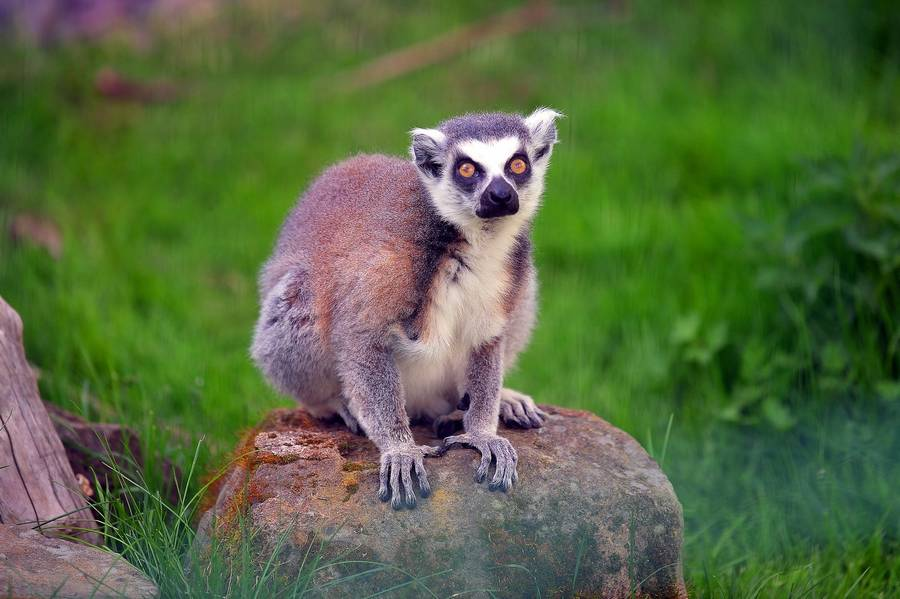
\includegraphics[width=\textwidth]{lemur.jpg}
    \caption{Oryginalny obrazek}
    \label{fig:lemur}
\end{figure}

\section{Grayscale}

Do konwersji obrazka na skalę szarości użyłem kowolucji. Jako wartość
szarości została wybrana średnia z wartości RGB. Domyślne wartości to:
padding=0, stride=1. Widoczne na obrazku \ref{fig:lemur_grayscale}.

\begin{lstlisting}
conv = nn.Conv2d(3, 1, kernel_size=1, bias=False)
conv.weight = nn.Parameter(torch.ones(1, 3, 1, 1) / 3)
grayscale = conv(tensor.unsqueeze(0)).squeeze(0)
\end{lstlisting}

\begin{figure}[H]
    \centering
    \includegraphics[width=\textwidth]{lemur_grayscale.png}
    \caption{Oryginalny obrazek w skali szarości}
    \label{fig:lemur_grayscale}
\end{figure}

\section{Zmniejszenie rozmiaru obrazka}

Do zmniejszenia obrazka użyłem poolingu maksymalnego. W przypadku krawędzi
zależałoby nam, żeby  jasny obszar pozostał bardzo jasny, a nie był ściemniany
przez okoliczne piksele. Wydaje się, że max pooling jest w tym przypadku
lepszy niż average pooling. Widoczne na obrazku \ref{fig:lemur_grayscale_small}.

\begin{figure}[H]
    \centering
    \includegraphics[width=\textwidth]{lemur_pooled.png}
    \caption{Obrazek w skali szarości o dwukrotnie mniejszym rozmiarze}
    \label{fig:lemur_grayscale_small}
\end{figure}

\section{Filtr Gaussa}

Użyłem filtru Gaussa o rozmiarze 7x7 i odchyleniu standardowym 1.
Doszedłem do tych wartości eksperymentalnie.
Maskę tworzyłem w następujący sposób:

\begin{lstlisting}
def gauss_kernel(size, sigma=1):
    kernel = torch.zeros(1, 1, size, size)
    half_size = size // 2
    double_sigma_sq = 2 * sigma**2
    for i in range(size):
        for j in range(size):
            kernel[0, 0, i, j] = exp(
                -((i - half_size) ** 2 + \
                (j - half_size) ** 2) / (double_sigma_sq)
            )
    return kernel / kernel.sum()
\end{lstlisting}

Wynik tej operacji przedstawiłem na obrazku \ref{fig:lemur_gauss}.

\begin{figure}[H]
    \centering
    \includegraphics[width=\textwidth]{lemur_gauss.png}
    \caption{Obrazek po zastosowaniu filtru Gaussa}
    \label{fig:lemur_gauss}
\end{figure}

\section{Gradienty}

W dalszej kolejności zastosowałem filtry Sobela. Implementacja poniżej:
\begin{lstlisting}
sob_vert = torch.FloatTensor([[1, 2, 1], [0, 0, 0], [-1, -2, -1]])
sob_hori = torch.FloatTensor([[1, 0, -1], [2, 0, -2], [1, 0, -1]])

conv = nn.Conv2d(1, 2, kernel_size=3, stride=1, bias=False)
conv.weight = nn.Parameter(torch.stack([sob_vert.unsqueeze(0), sob_hori.unsqueeze(0)]))
sobel = conv(gauss.unsqueeze(0)).squeeze(0)
\end{lstlisting}

Rysunek
\ref{fig:lemur_grad} przedstawia gradienty w obu kanałach.

\begin{figure}[H]
    \centering
    \includegraphics[width=\textwidth]{lemur_sobel.png}
    \caption{Gradienty obrazka}
    \label{fig:lemur_grad}
\end{figure}

Dane z obu kanałów połączyłem w jeden kanał intensywności,
używając normy euklidesowej. Można ten etap zobaczyć na obrazku
\ref{fig:lemur_grad_norm}.

\begin{figure}[H]
    \centering
    \includegraphics[width=\textwidth]{lemur_intensity.png}
    \caption{Norma gradientów obrazka}
    \label{fig:lemur_grad_norm}
\end{figure}

Do liczenia kąta użyłem funkcji torch.atan2.

\section{ Wykrywanie krawędzi }

Do sprawdzania czy dany piksel jest krawędzią użyłem poniższej implementacji:

\begin{lstlisting}
def non_max_supression(intensity, angle):
    assert intensity.shape == angle.shape
    assert intensity.dim() == 2

    max_intensity = intensity.max()
    height, width = intensity.shape

    # create output tensor
    output = torch.zeros(height, width)

    for i in range(height):
        for j in range(width):

            try:
                a = max_intensity
                b = max_intensity
                # 0 degrees
                current_angle = angle[i, j]
                if current_angle < 22.5 or current_angle > 157.5:
                    a = intensity[i, j + 1]
                    b = intensity[i, j - 1]
                # 45 degrees
                elif 22.5 < current_angle < 67.5:
                    a = intensity[i + 1, j + 1]
                    b = intensity[i - 1, j - 1]
                # 90 degrees
                elif 67.5 < current_angle < 112.5:
                    a = intensity[i + 1, j]
                    b = intensity[i - 1, j]
                # 135 degrees
                elif 112.5 < current_angle < 157.5:
                    a = intensity[i - 1, j + 1]
                    b = intensity[i + 1, j - 1]

                if intensity[i, j] >= a and intensity[i, j] >= b:
                    output[i, j] = intensity[i, j]

            except IndexError:
                pass
    return output / output.max()
\end{lstlisting}

Wynik tej operacji przedstawiłem na obrazku \ref{fig:lemur_edges}.

\begin{figure}[H]
    \centering
    \includegraphics[width=\textwidth]{lemur_non_max.png}
    \caption{Wykryte krawędzie}
    \label{fig:lemur_edges}
\end{figure}

\section{Progowanie}

W tym kroku wartości mniejsze niż dany próg zostały ustawione na 0, a większe
zostały ustawione na 1. Testowane dla różnych wartości progu. Widoczne na obrazku
\ref{fig:lemur_threshold}. W porówaniu do oryginalnej metody Canny'ego, tutaj
stosujemy jedynie jeden próg, a nie dwa. Spowoduje to, że nasze krawędzie będą
urywane w miejscach, gdzie jest nadal krawędź, ale nie tak wyraźna.

\begin{figure}[H]
    \centering
    \includegraphics[width=\textwidth]{lemur_threshold.png}
    \caption{Wykryte krawędzie}
    \label{fig:lemur_threshold}
\end{figure}

\section{Wynik}

Na koniec oryginalny obraz i krawędzie nałożyłem na siebie dodając je.
Znalezione krawędzie są widoczne na obrazku \ref{fig:lemur_result}.
Część możemy uznać na nieważne, ale większość "chcianych" krawędzi
została wykryta. Większość znalezionych krawędzi ma sens.

\begin{figure}[H]
    \centering
    \includegraphics[width=\textwidth]{lemur_result.png}
    \caption{Wynik}
    \label{fig:lemur_result}
\end{figure}

Dla porównania tutaj wynik z biblioteki OpenCV z progami 100 i 200:

\begin{figure}[H]
    \centering
    \includegraphics[width=\textwidth]{lemur_cv.png}
    \caption{Wynik z OpenCV}
    \label{fig:lemur_cv}
\end{figure}



\end{document}
